\documentclass{article}
\usepackage[english]{babel}
\usepackage{amsmath}
\usepackage{graphicx}
\usepackage{float}
%\usepackage{algorithmicx}
\usepackage{algpseudocode}

\title{Clustering big data}
\author{Dan Filimon}

\begin{document}
\maketitle

\tableofcontents

\pagebreak

\section{Rationale}

Telescopes surveying the Universe in search of exoplanets, DNA sequencers
decoding our genes, governments monitoring cities, and people all over the
world exchanging messages, images, videos produce across the Internet produce
exabytes of data every day.

Researchers, businesses and governments all over the world are trying to make
sense of the ever-increasing collection of data they have access to.

It needs to be stored, searched through, processed and analyzed to extract
valuable information.
Such a large volume of data comes with its own set of challenges and in the
past few years, novel programming paradigms have emerged that make analyzing
this data a lot more accessible.
There are many systems that are designed to handle ``big data''. Out of these, the most famous one is MapReduce \cite{mr1} from Google, for batch
processing and more recently Storm \cite{st1} originally from Backtype, now acquired by
Twitter.

Many applications that have previously been impossible are now a reality thanks
to massive data sets. For example, quality statistical machine Translation can only
work at very large scale. While the accuracy of currently available commerical
fails to capture more subtle nuances, it is certainly good enough to convey the
general meaning.

Large scale data analysis is a broad field with many overlapping disciplines
like machine learning, data mining, data science etc.

Analyzing big data is challening. The complexity of many algorithms makes them
difficult to parallelize and even when this is possible, because of the scale
of the data, clusters of many machines are needed to process the data in
reasonable time.

The mainframe era of the 80s, displaced by the affordable
personal computer is making a comeback under the guise of ``cloud computing''
precisely because the complexity of maintaining a large enough cluster of machines
to process ``big data'' makes it a ripe target for outsourcing.

Companies now offer ``clouds'', clusters of virtual machines that support
MapReduce style processing through open-source Hadoop distributions like Amazon
(Amazon Web Services), Google (Google Compute Engine), Microsoft (Windows
Azure) have vast data centers at their disposal and offer infrastructure as a
service to be billed by the hour (or minute).

Time is quite literally money in this market which makes fast processing even
more critical. When processing data at terrabye scale and beyond especially in
pipelines, the first priority is usually to reduce the data through some
aggregation such that the resulting size is much smaller, for example storing
statistics instead of the raw data.

One of the most useful algorithms to analyze data with is clustering.
Intuitively the aim of clustering is to find clumps of data that are more
similar to one another than the others.

The traditional use of clustering is for revealing interesting patterns in the
data --- for example, if $n$ good quality clusters do form, this could mean there
are $n$ types of users in the system.

It's also especially useful for getting a good representative sample of the data
that should behave similarly to the original distribution.
This is important because sometimes there are no obvious ways of aggregating the
data being processed directly to reduce its size. If the data is clustered
however, the resulting clusters' centroids can be used as input for the next
stage of processing.

\section{Clustering}

There are many kinds of clustering which vary significantly in their approach
in building the clusters. The kind of clustering we'll be discussing in this
paper is ``centroid'' based.

To apply any clustering, or machine learning for that matter, the data needs to
be transformed from its raw representation to ``feature vectors''. The
corresponding feature vector for a data item should capture plausibly relevant
characteristics of the item in a numeric form.
For example, when working with text documents, feature vectors containing
frequencies a given word in a document compared to the corpus are useful.

This paper doesn't attempt to further describe the various ways used to encode
data into feature vectors or assess the usefulness of a subset of features.
This is requires domain-specific knowledge and is the goal of feature engineering.
It's assumed the data is already available as feature vectors and so now
the clustering problem can be formalized.

Given $n$ vectors (also referred to as a points) in $\textbf{R}^d$ and an
integer $k$, and a distance measure, $dist$, group the $n$ points
into $k$ disjoint sets $X_1$ through $X_k$. The mean of
the points in cluster $i$ (or, disjoint set $X_i$) is called the ``centroid''
of that cluster, which we call $c_i$.

The clustering needs to be good in some sense, so define a measure of
quality to optimize for. For this, $dist$, a distance measure is needed, making the combined vector space and measure a metric space.

$T_c$, is what gets optimized for --- the total cost of the clustering, which is the sum of the distances
from each point to the centroid of the cluter it is assigned to.

\begin{eqnarray}
    T_c = \sum_{i = 1}^{k} \left( \sum_{\bf x_{ij} \in X_i} dist({\bf x_{ij}},
    {\bf c_i})
    \right)
\end{eqnarray}

In this formulation, the number of clusters, $k$ is fixed, but this problem is
related to the facility placement problem, which essentially identical except
in that the number of cluster can vary.

The main issue with this formulation is that the optimization problem we're
trying to solve is NP-hard in the general case.
This has the very important implication that it is infeasible to find an
optimal solution to this problem. Any polynomial-time algorithm we can devise
will at best be an approximation scheme.
This turns out to not be as dire as it first sounds, because ``good enough'' is
fine for virtually all applications and also because real data tends to have
additional properties that results in stronger quality guarantees.

\subsubsection{Distance measure}
One difference users used to clustering literature might have noticed in this
formulation is that our
choice of distance measure is not fixed. Normally most papers on clustering
work with $||{\bf x - y}||_2^2$, the squared Euclidean distance (or squared
$L2$-norm). We acknowledge this and indeed some results we use for our
implementations have this assumption. As implementors of a machine learning
library however, we need to support user extensibility and we feel that other
than providing documentation to our users, we shouldn't enforce other kinds of
restrictions. It turns out that most distances used in practice
are variants of this distance measure (for example the $L2$-norm and the cosine
distance), in which case the results likely the same. If some completely
different distance measure is used, we can't provide any guarantees.

\subsection{Quality}

When it comes to the quality of the clusters generated by any algorithm, it is
often said that ``clustering is in the eye of the beholder''.
In unsupervised learning, which this problem is a part of, there is no
known ``right answer''. Compare this with classification or regression where an
example is either correctly clasified or predicted, or it isn't.

Things are not so clear-cut in this case. While the total cost is certainly
what we optimize for, multiple measure have been devised over the years that
attempt to formalize the degree a clustering is ``good''.
Intuitively, we want clusters that are:
\begin{itemize}
    \item compact, meaning that the points in a cluster are close together (the
        intra-cluster distances are small between any two points)
    \item well separated, meaning that two different clusters will be
        relatively far apart (the inter-cluster distances are large between any
        two clusters)
\end{itemize}

The Dunn Index and Davies-Bouldin Index try to express compactness and
separability in one score. These are called ``internal'' scores because they
only at one clustering.

Additionally, it is often useful to compare two different clusterings and to
see how similar they are. This is useful especially when comparing different
clusteirng algorithms. A widely used score for this is the Adjusted Rand Index
based off the ``confusion matrix'' (same idea as with classification).

\subsubsection{Dunn Index}
The Dunn Index, was invented in 1974 by J. Dunn. A higher Dunn Index indicates
a better clustering. It combines $\Delta_i$, a distance score for cluster $i$
(called intracluster distance) and the distance between two clusters,
$dist(\mathbf{c}_i, \mathbf{c}_j)$ (intercluster distance).

$\Delta_i$ can have different expressions. For cluster $X_i$ it could be:
\begin{itemize}
    \item the maximum distance between any two points
        \begin{eqnarray}
            \Delta_i = \max_{\mathbf{x}, \mathbf{y} \in X_i} dist(\mathbf{x},
            \mathbf{y}) \;\textrm{}
        \end{eqnarray}
    \item the mean distance between any two points
        \begin{eqnarray}
            \Delta_i = \frac{1}{|X_i| (|X_i| - 1)} \sum_{\mathbf{x}, \mathbf{y} \in
            X_i, \mathbf{x} \ne \mathbf{y}} dist(\mathbf{x}, \mathbf{y})
        \end{eqnarray}
    \item the mean distance between any point and the centroid
        \begin{eqnarray}
            \Delta_i = \frac{\sum_{\mathbf{x} \in X_i} dist(\mathbf{x},
            \mathbf{c}_i)}{|X_i|}
        \end{eqnarray}
    \item the median distance between any point and the centroid. This is the
        one we use in the implementation. The reasoning is that the median is
        much more roubst to outliers than the mean or max. Additionally,
        computing distances between all pairs of points is simply not feasible
        for large datasets.
\end{itemize}

Having defined $\Delta_i$, the Dunn Index is:

\begin{eqnarray}
    D = \min_{1 \le i \le k} \left\{ \min_{1 \le j \le k, j \ne i} \left\{
        \frac{dist(\mathbf{c}_i, \mathbf{c}_j)}{\max_{1 \le l \le k} \Delta_l}
    \right\} \right\}
\end{eqnarray}

\subsubsection{Davies-Bouldin Index}
The Davies-Bouldin Index was invented in 1979 by D. Davies and D. Bouldin. Like
the Dunn Index, it is an internal evaluation scheme. A lower Davies-Bouldin
Index indicates a better clustering.

Defining a cluster-specific measure, exactly like for the Dunn Index,
$\Delta_i$, the index is:
\begin{eqnarray}
    DB = \frac{1}{k} \sum_{i = 1}^k \max_{j \ne i} \left( \frac{\Delta_i +
    \Delta_j}{dist(\mathbf{c}_i, \mathbf{c}_j)} \right)
\end{eqnarray}

\subsubsection{Adjusted Rand Index}
The Rand Index was invented by W. Rand in 1971. It measures how similar two
clusterings are to one another. When the index is adjusted for change grouping
of elements it is known as the Adjusted Rand Index.

To compute the index, one must first construct a contingency table (also known
as a confusion matrix). Assuming the clusterings are $X = \{X_1, X_2, \ldots
X_k\}$ and $Y = \{Y_1, Y_2, \ldots Y_k\}$, the overlap between cluster $i$ of
$X$, and cluster $j$ of $Y$, $n_{ij}$ is the number of points that are closest
to cluster $i$ in clustering $X$ and cluster $j$ in clustering $Y$. That is
$n_{ij} = X_i \cap Y_j$.

\begin{center}
    \begin{tabular}{c | c  c  c  c | c}
        & $Y_1$ & $Y_2$ & $\ldots$ & $Y_k$ & Sums \\
        \hline
        $X_1$ & $n_{11}$ & $n_{12}$ & $\ldots$ & $n_{1k}$ & $a_1$ \\
        $X_2$ & $n_{21}$ & $n_{22}$ & $\ldots$ & $n_{2k}$ & $a_2$ \\
        $\vdots$ & $\vdots$ & $\vdots$ & $\ddots$ & $\vdots$ & $\vdots$ \\
        $X_k$ & $n_{k1}$ & $n_{k2}$ & $\ldots$ & $n_{kk}$ & $a_k$ \\
        \hline
        Sums & $b_1$ & $b_2$ & $\ldots$ & $b_k$ & \\
    \end{tabular}
\end{center}

The Adjusted Rand Index is:

\begin{eqnarray}
    AR = \frac{\sum_{ij} \left( \frac{n_{ij}}{2} \right) - \left[\sum_i
        \left( \frac{a_i}{2} \right) \sum_j \left( \frac{b_j}{2} \right)
        \right]/\left( \frac{n}{2} \right)}{\frac{1}{2} \left[ \sum_i \left(
            \frac{a_i}{2} \right) + \sum_j \left( \frac{b_j}{2} \right) \right] - \left[\sum_i
        \left( \frac{a_i}{2} \right) \sum_j \left( \frac{b_j}{2} \right)
        \right]/\left( \frac{n}{2} \right)}
\end{eqnarray}

\section{k-means}

The most famous, simple and quite venerable clustering algorithm, known since the 50s
is k-means and later Lloyd's method.

It first starts by chosing $k$ point out of the $n$ as seeds. These will be the
first centroids (they're not ``really'' centroids since they are not the means
of the points).
The algorithm then proceeds by doing some number of iterations of the following
steps:
\begin{enumerate}
    \item assign each point to the cluster whose centroid is closest to it
    \item recompute the existing centroids
\end{enumerate}
The following 6 figures illustrates how this works in a toy example with 2D
points we want to cluster into 3 clusters.

\begin{figure}[H]
    \caption{These are some example points we'll cluster in 3 groups}
    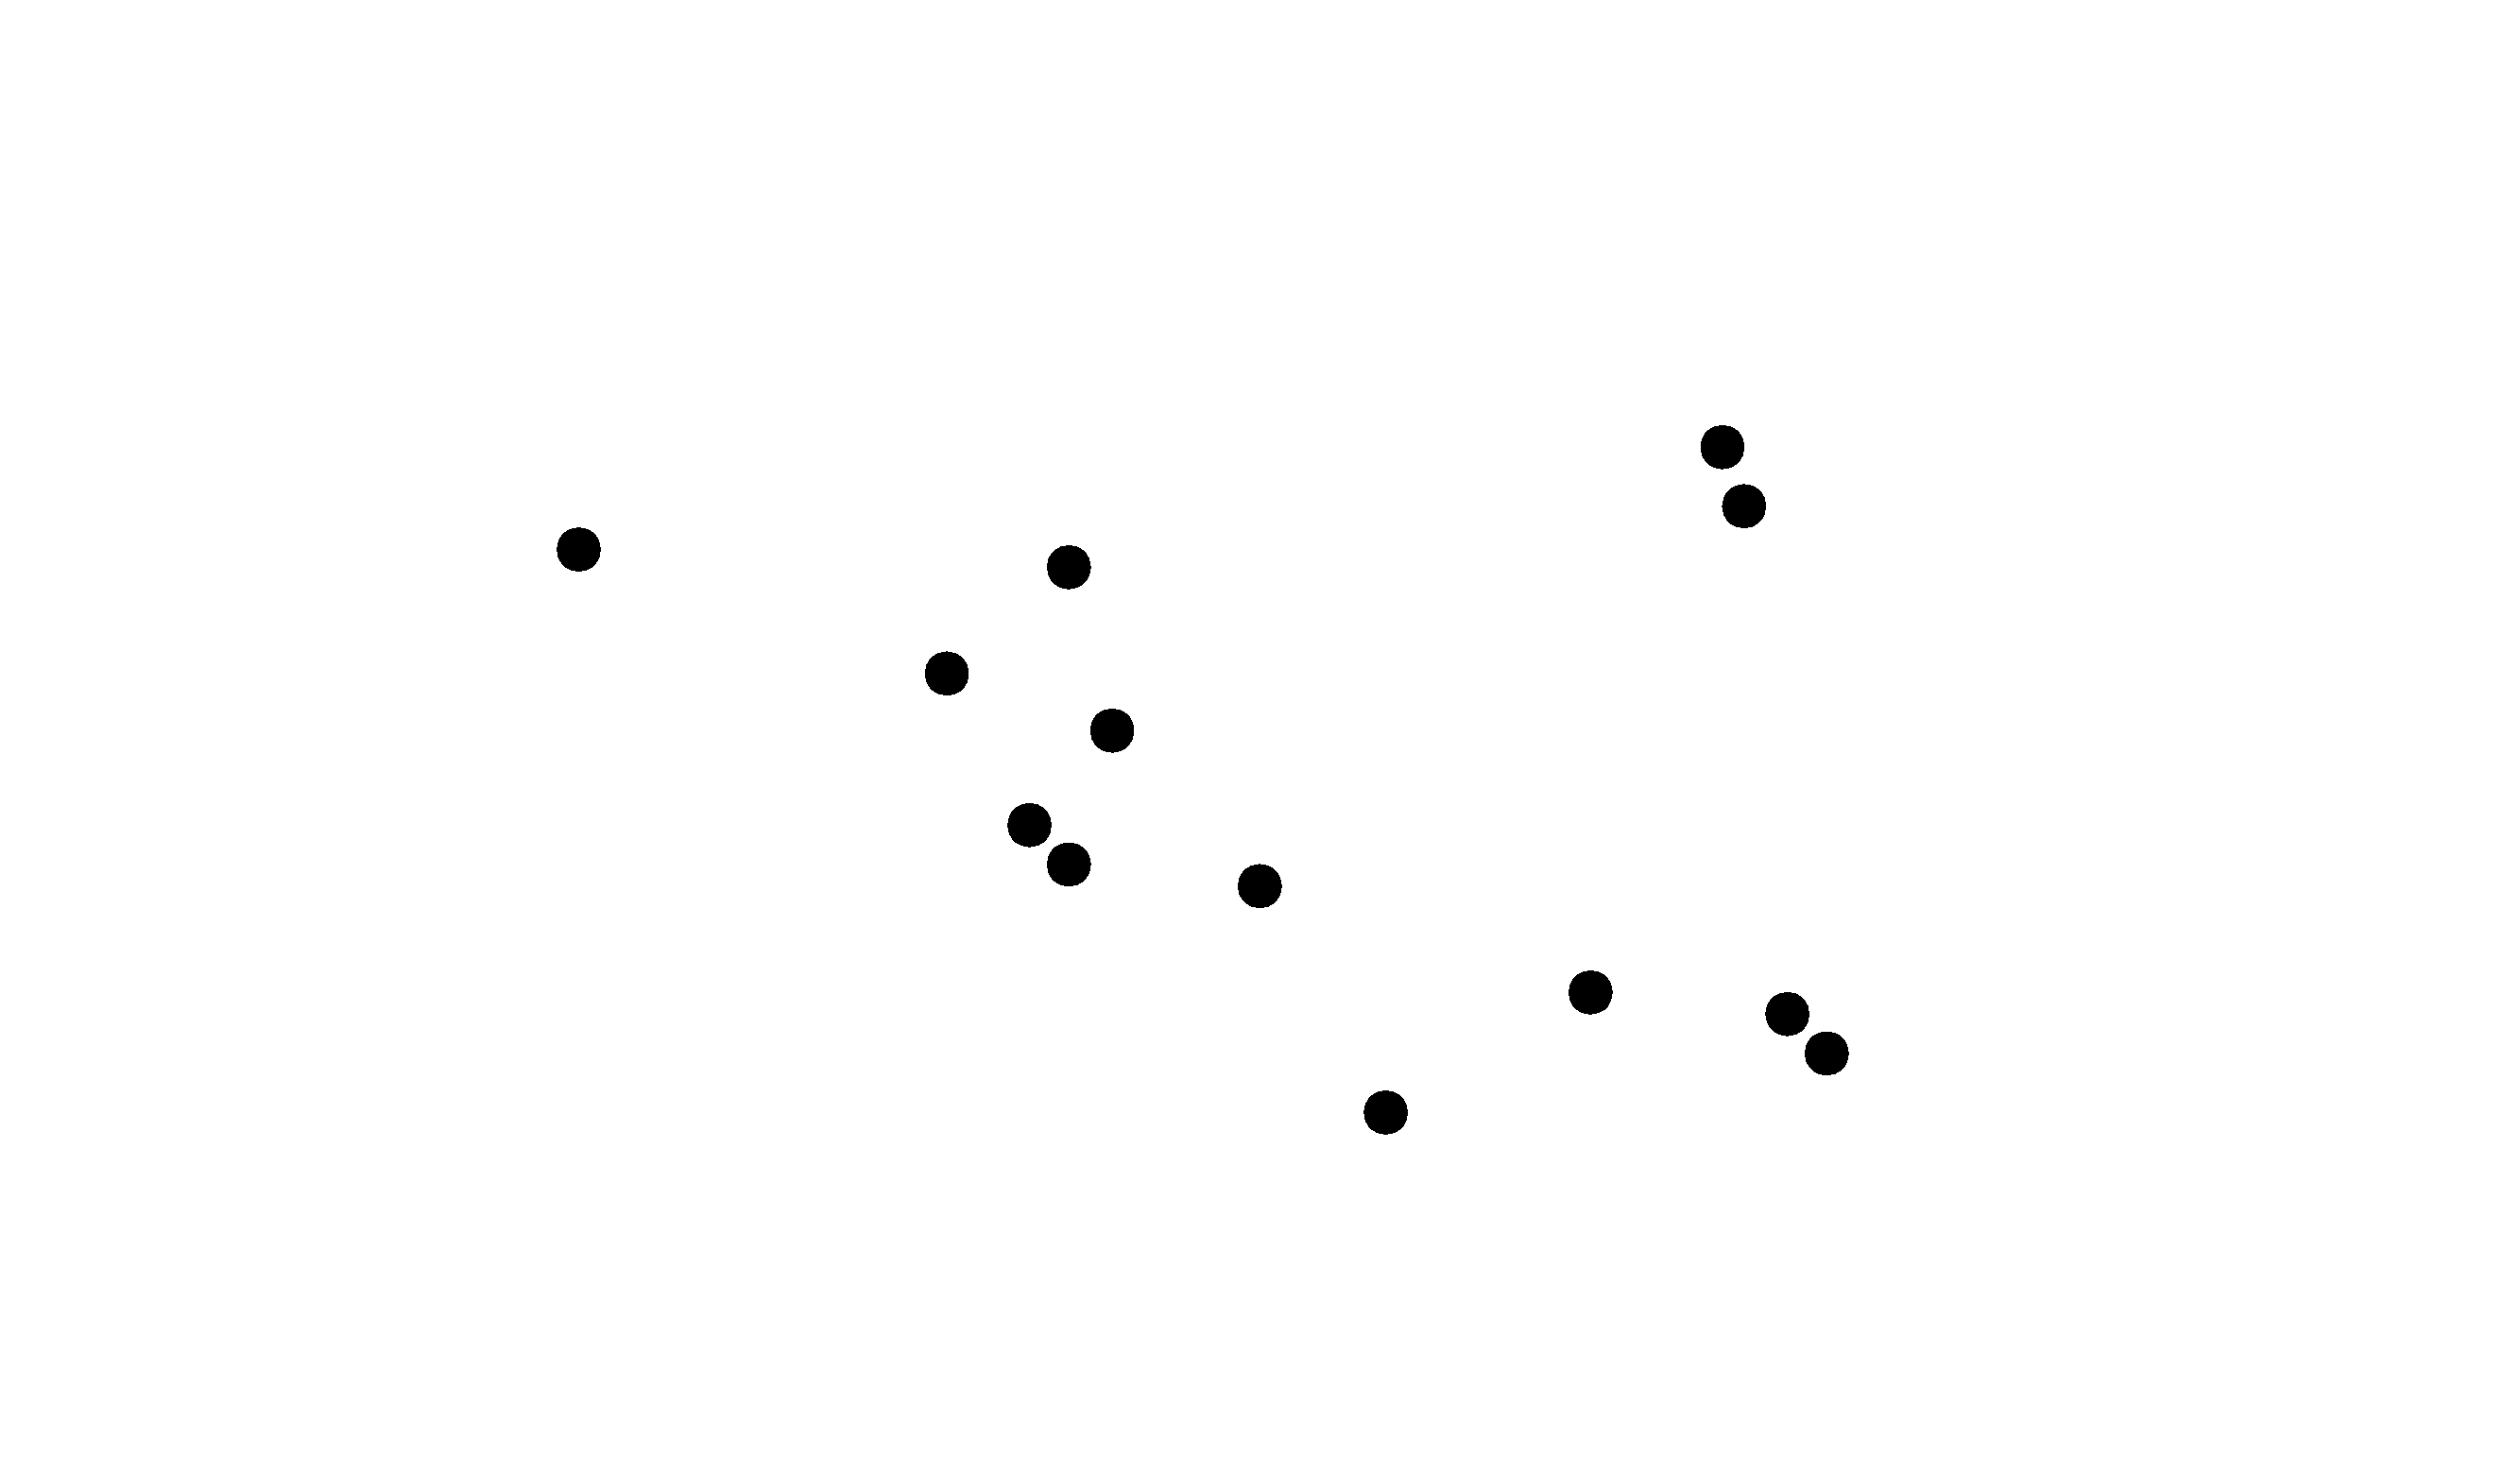
\includegraphics[scale=0.4]{kmeans-points-pre.pdf}
\end{figure}

\begin{figure}[H]
    \caption{Here we selected 3 points as the initial centroids}
    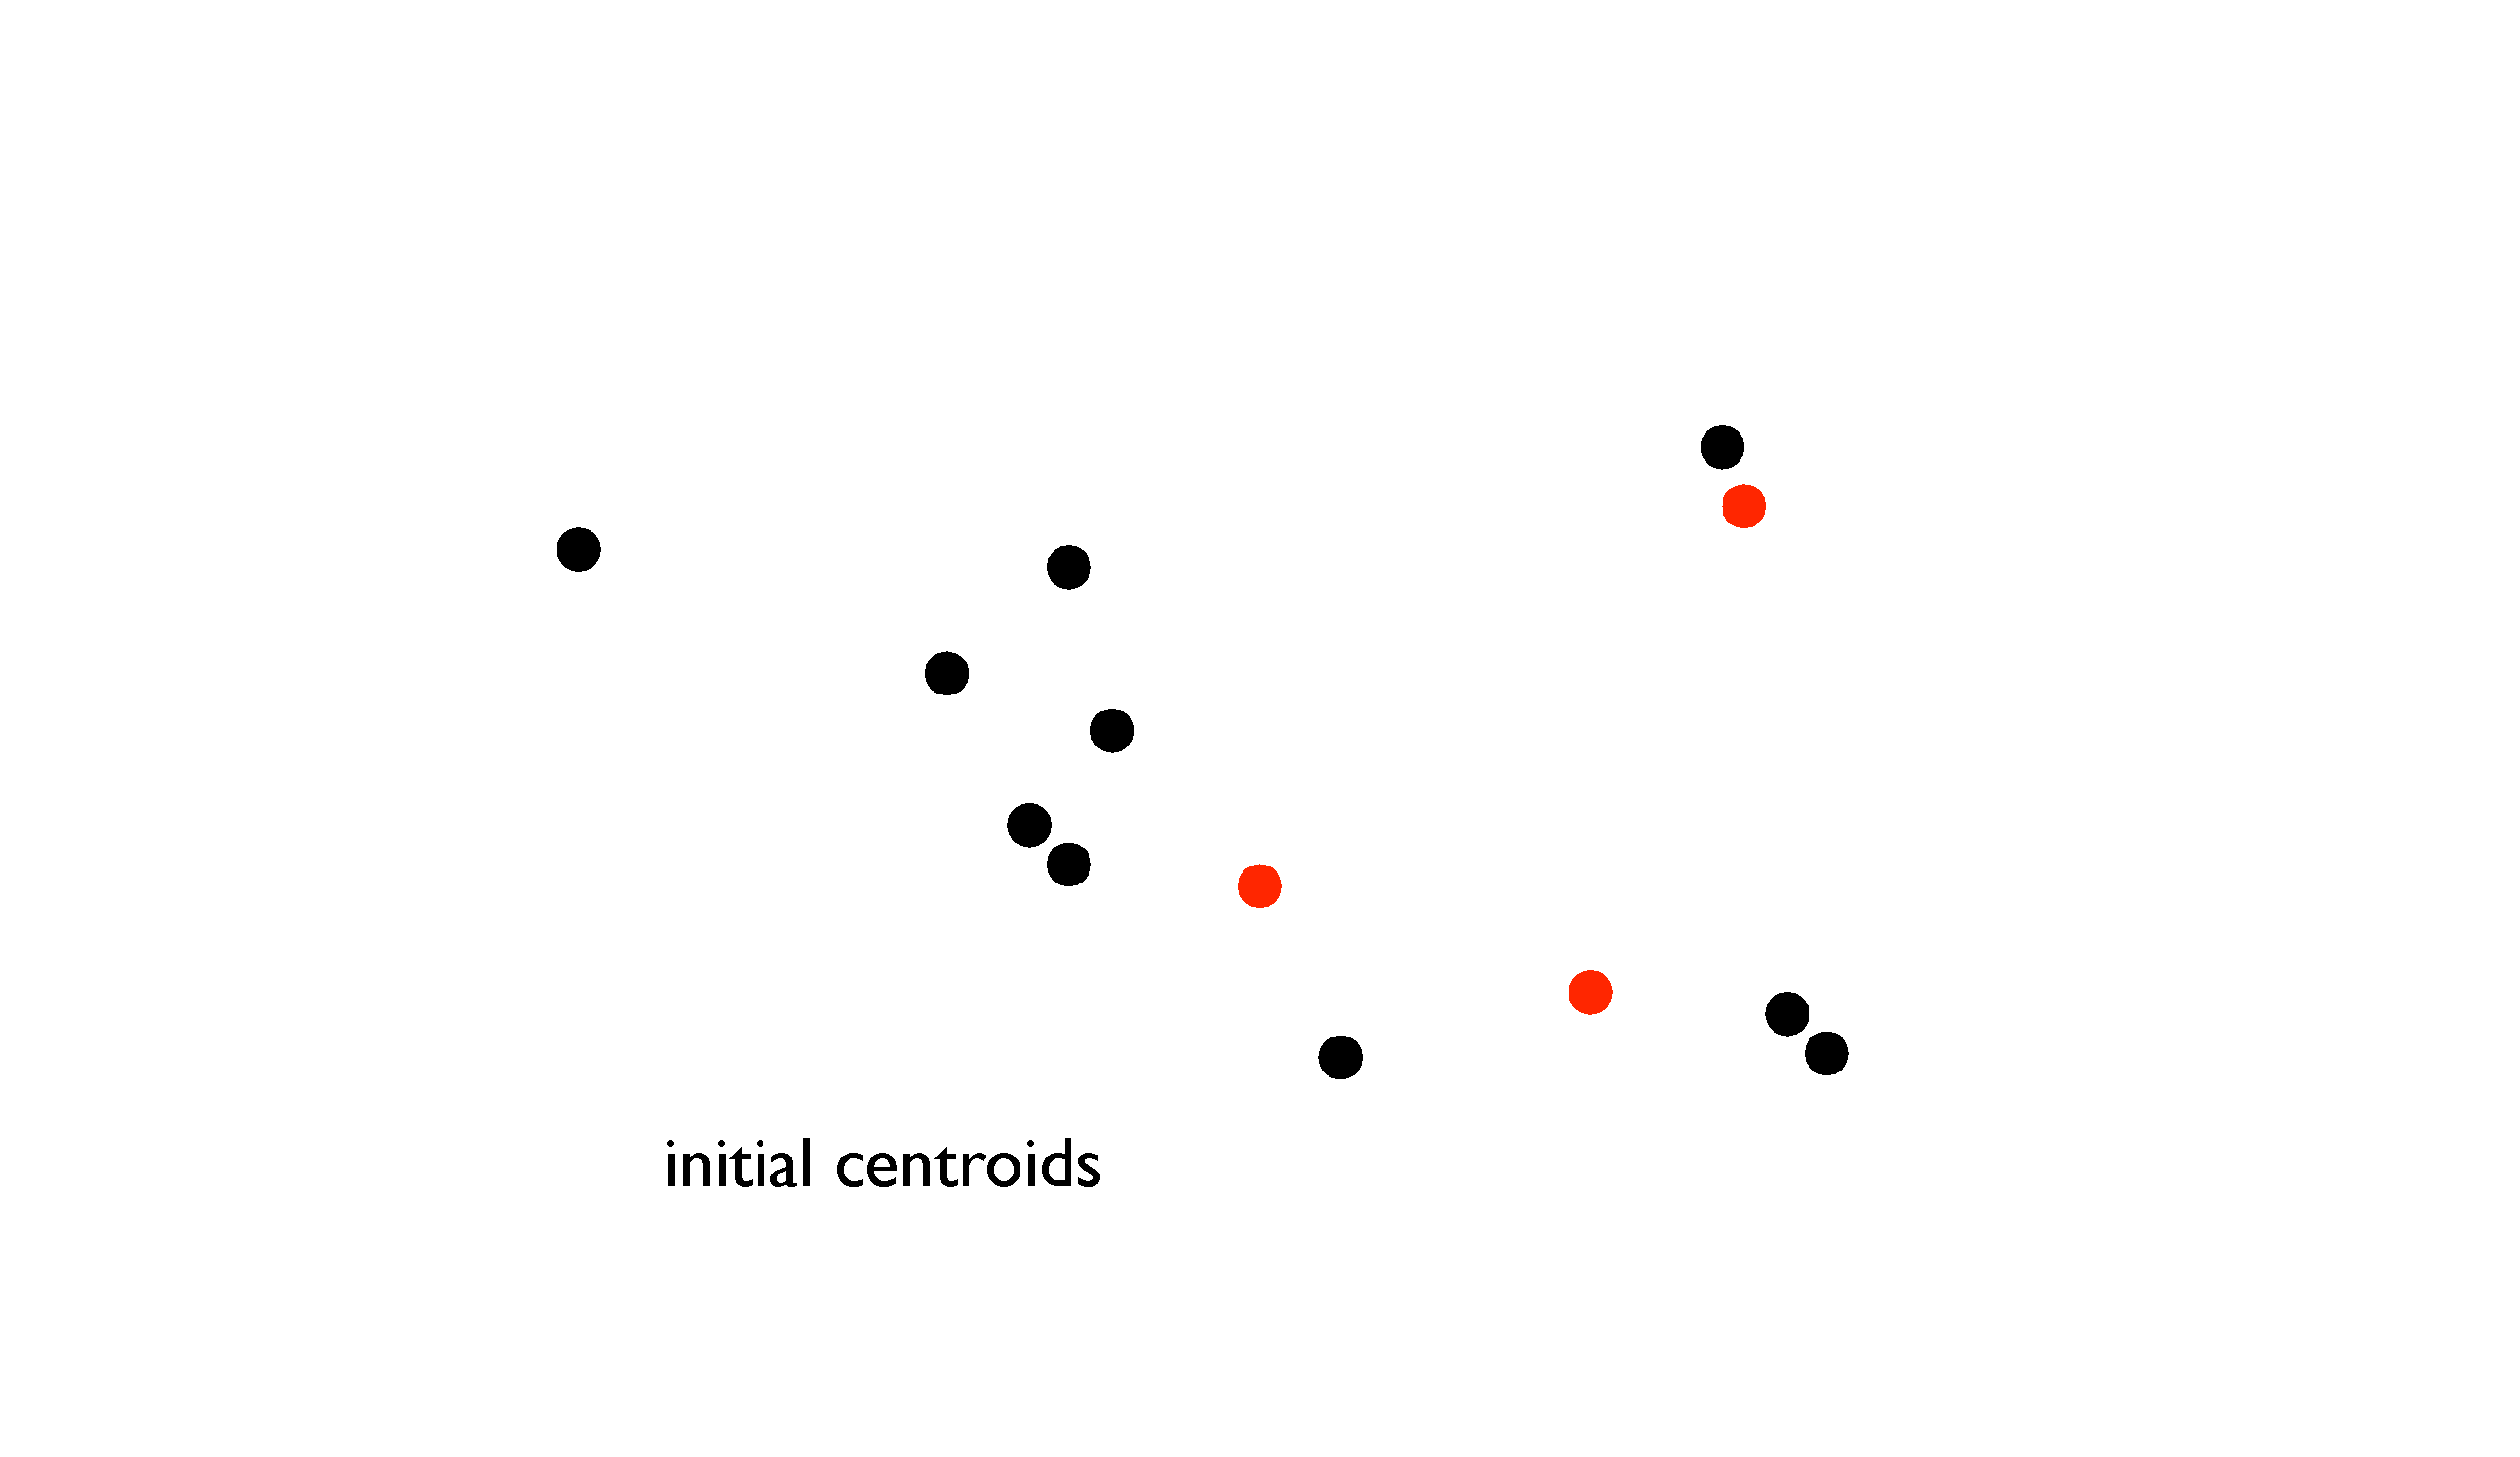
\includegraphics[scale=0.4]{kmeans-points-init.pdf}
\end{figure}

\begin{figure}[H]
    \caption{Here we assign each point to the cluster whose centroid it's
    closest to}
    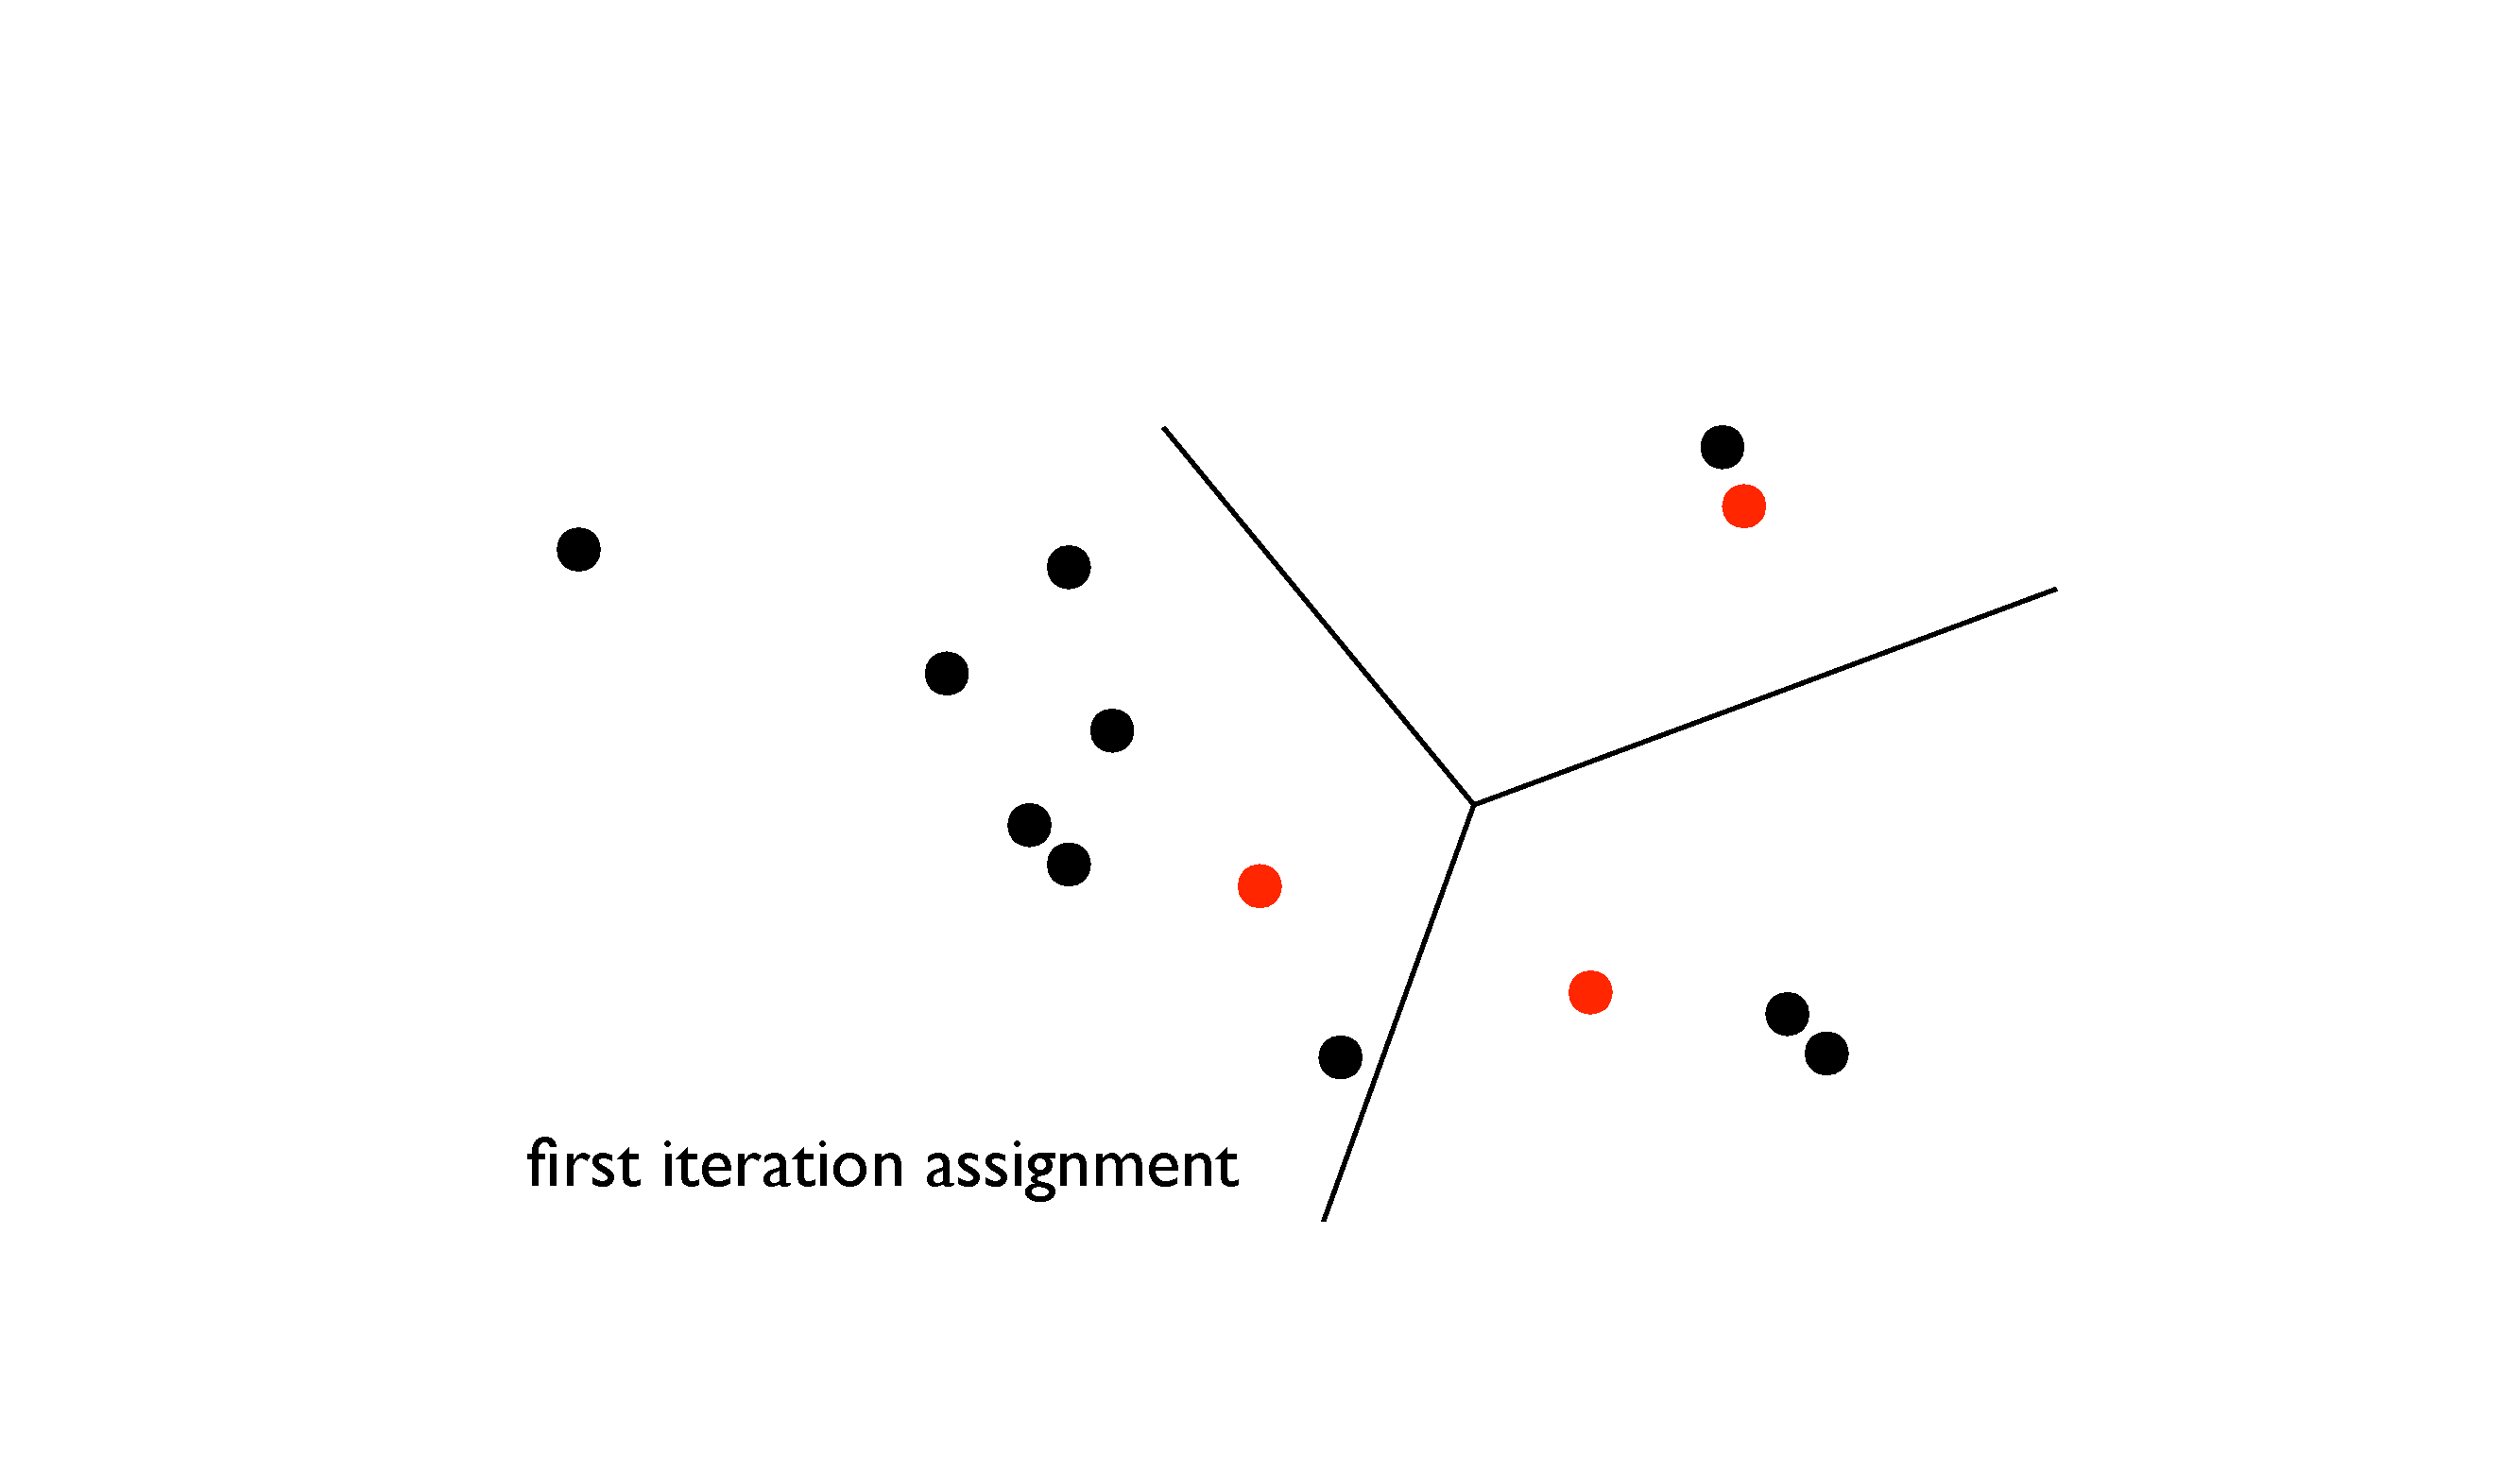
\includegraphics[scale=0.4]{kmeans-points-assign1.pdf}
\end{figure}

\begin{figure}[H]
    \caption{After asigning each point to a cluster, we compute the centroids
    of those clusters as the mean of the points in that cluster}
    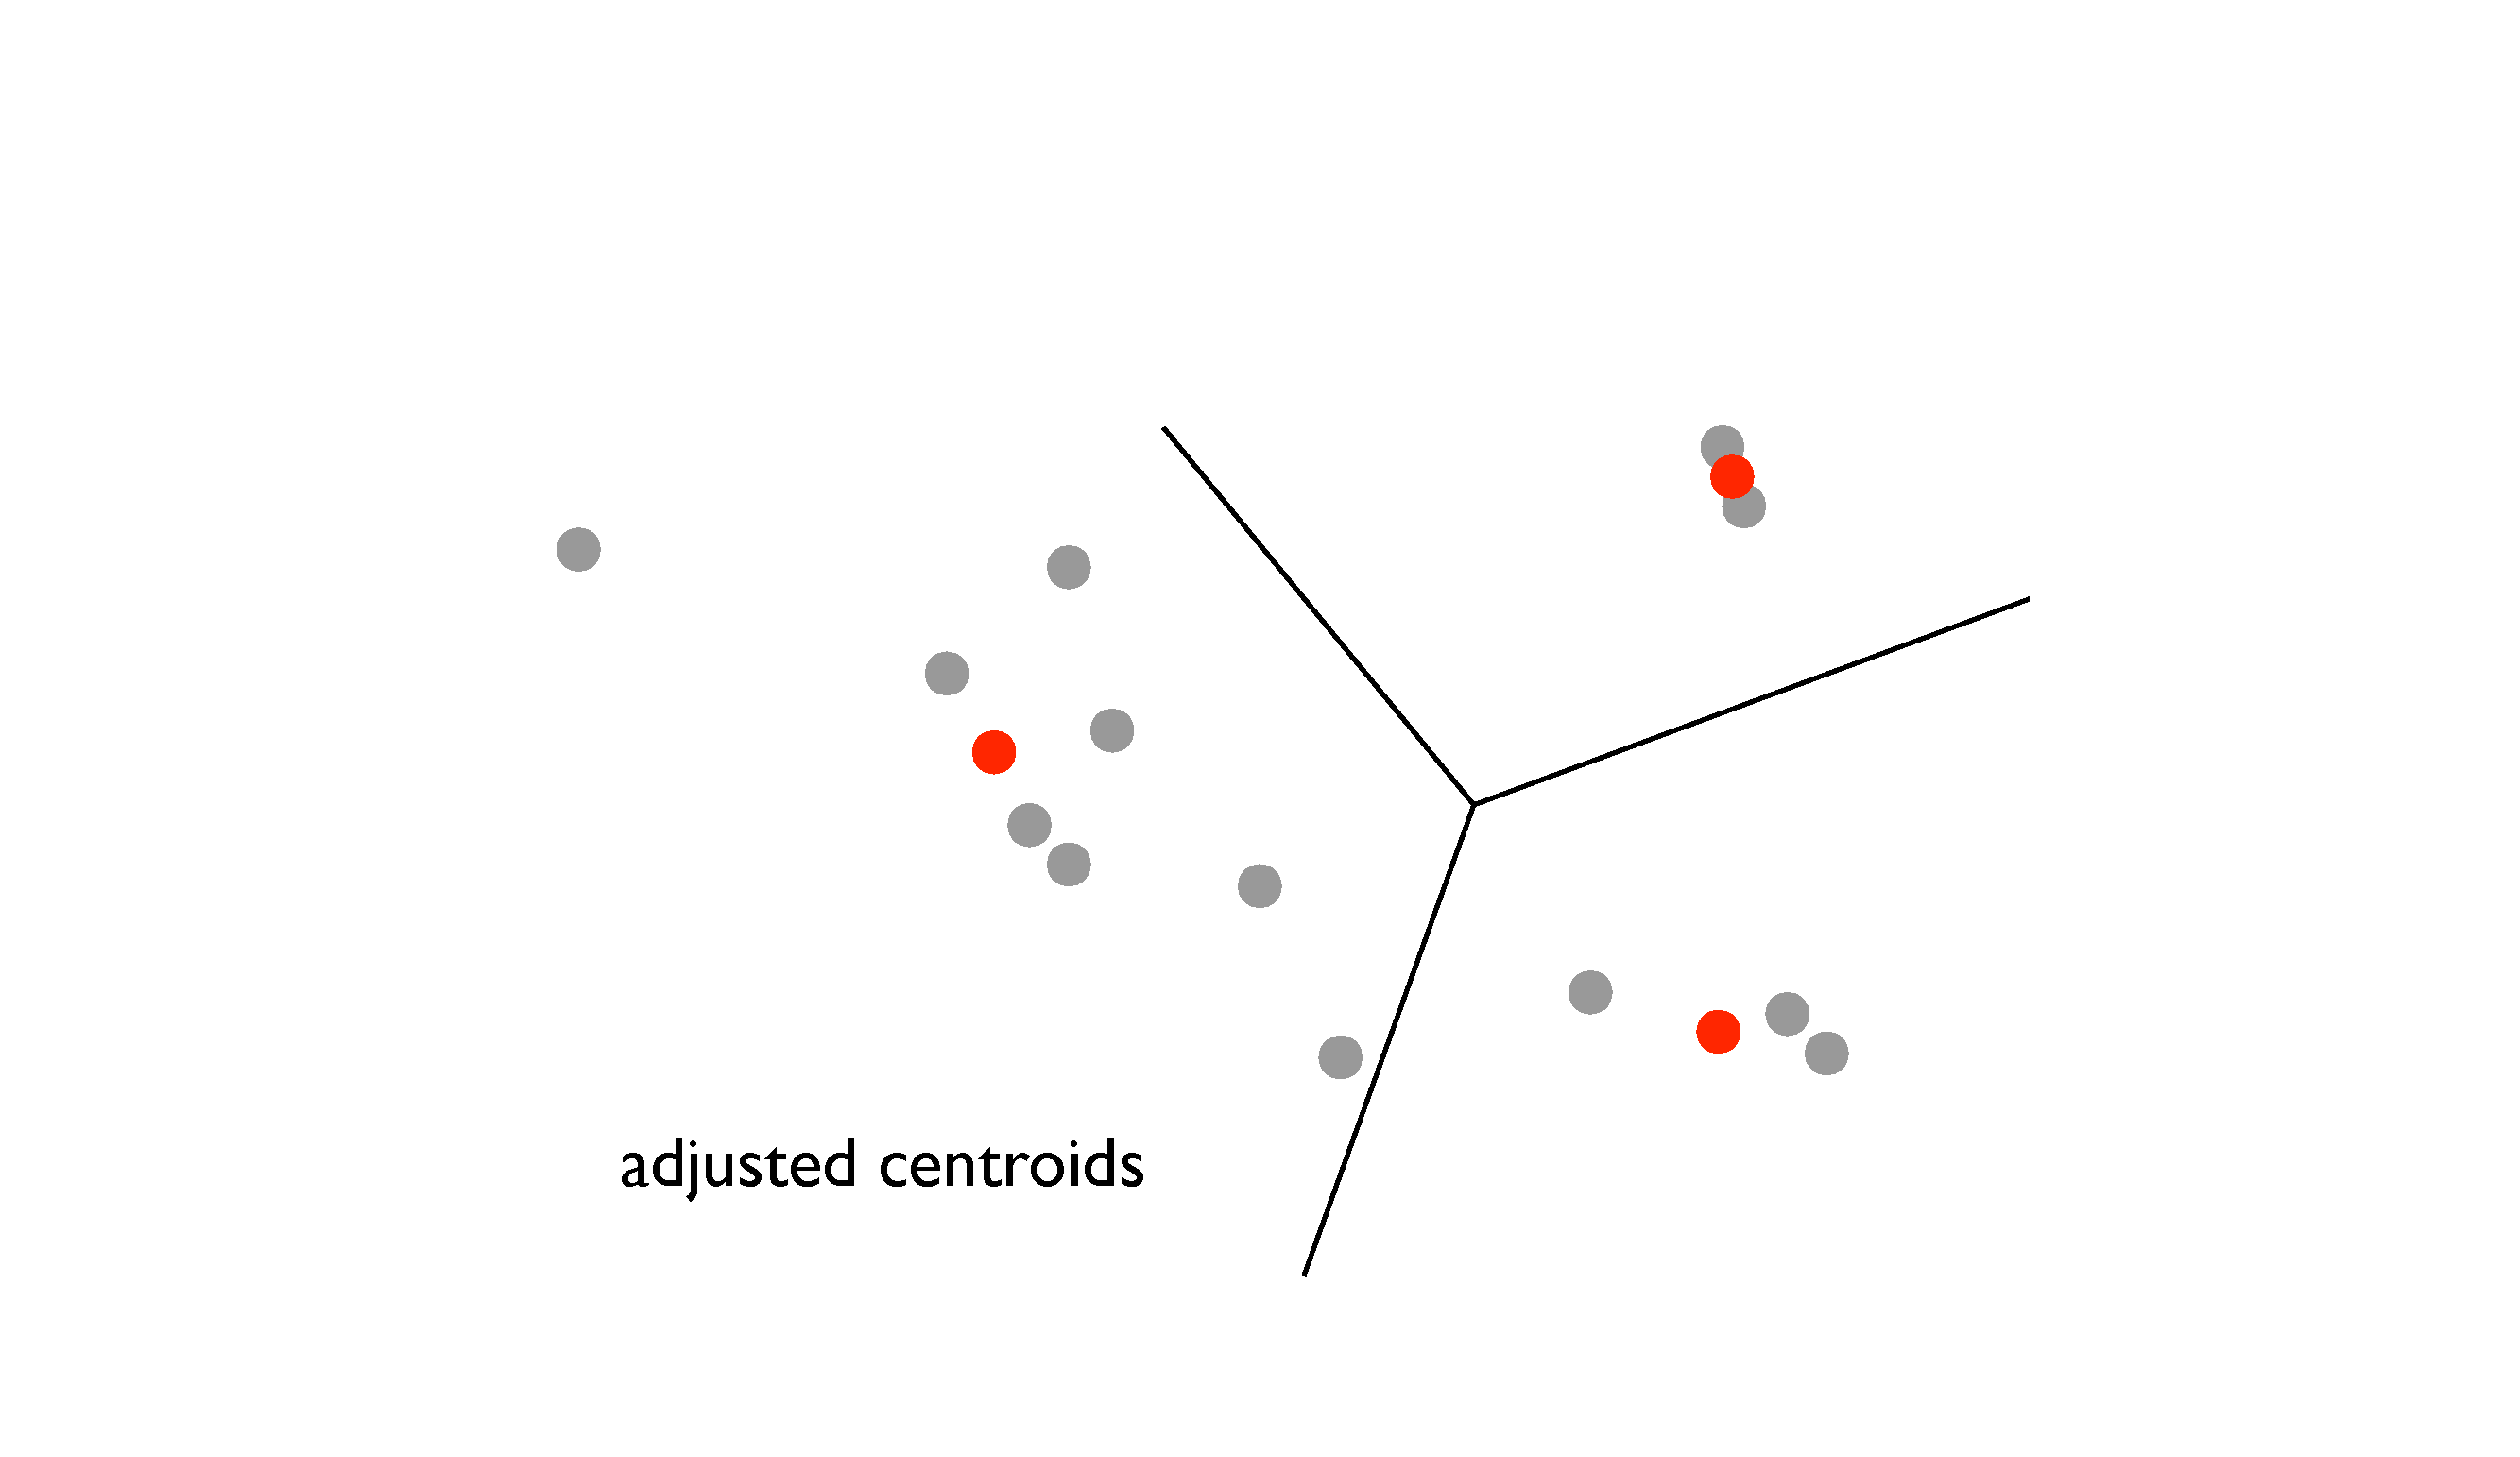
\includegraphics[scale=0.4]{kmeans-points-adjust1.pdf}
\end{figure}

\begin{figure}[H]
    \caption{Second iteration assignment}
    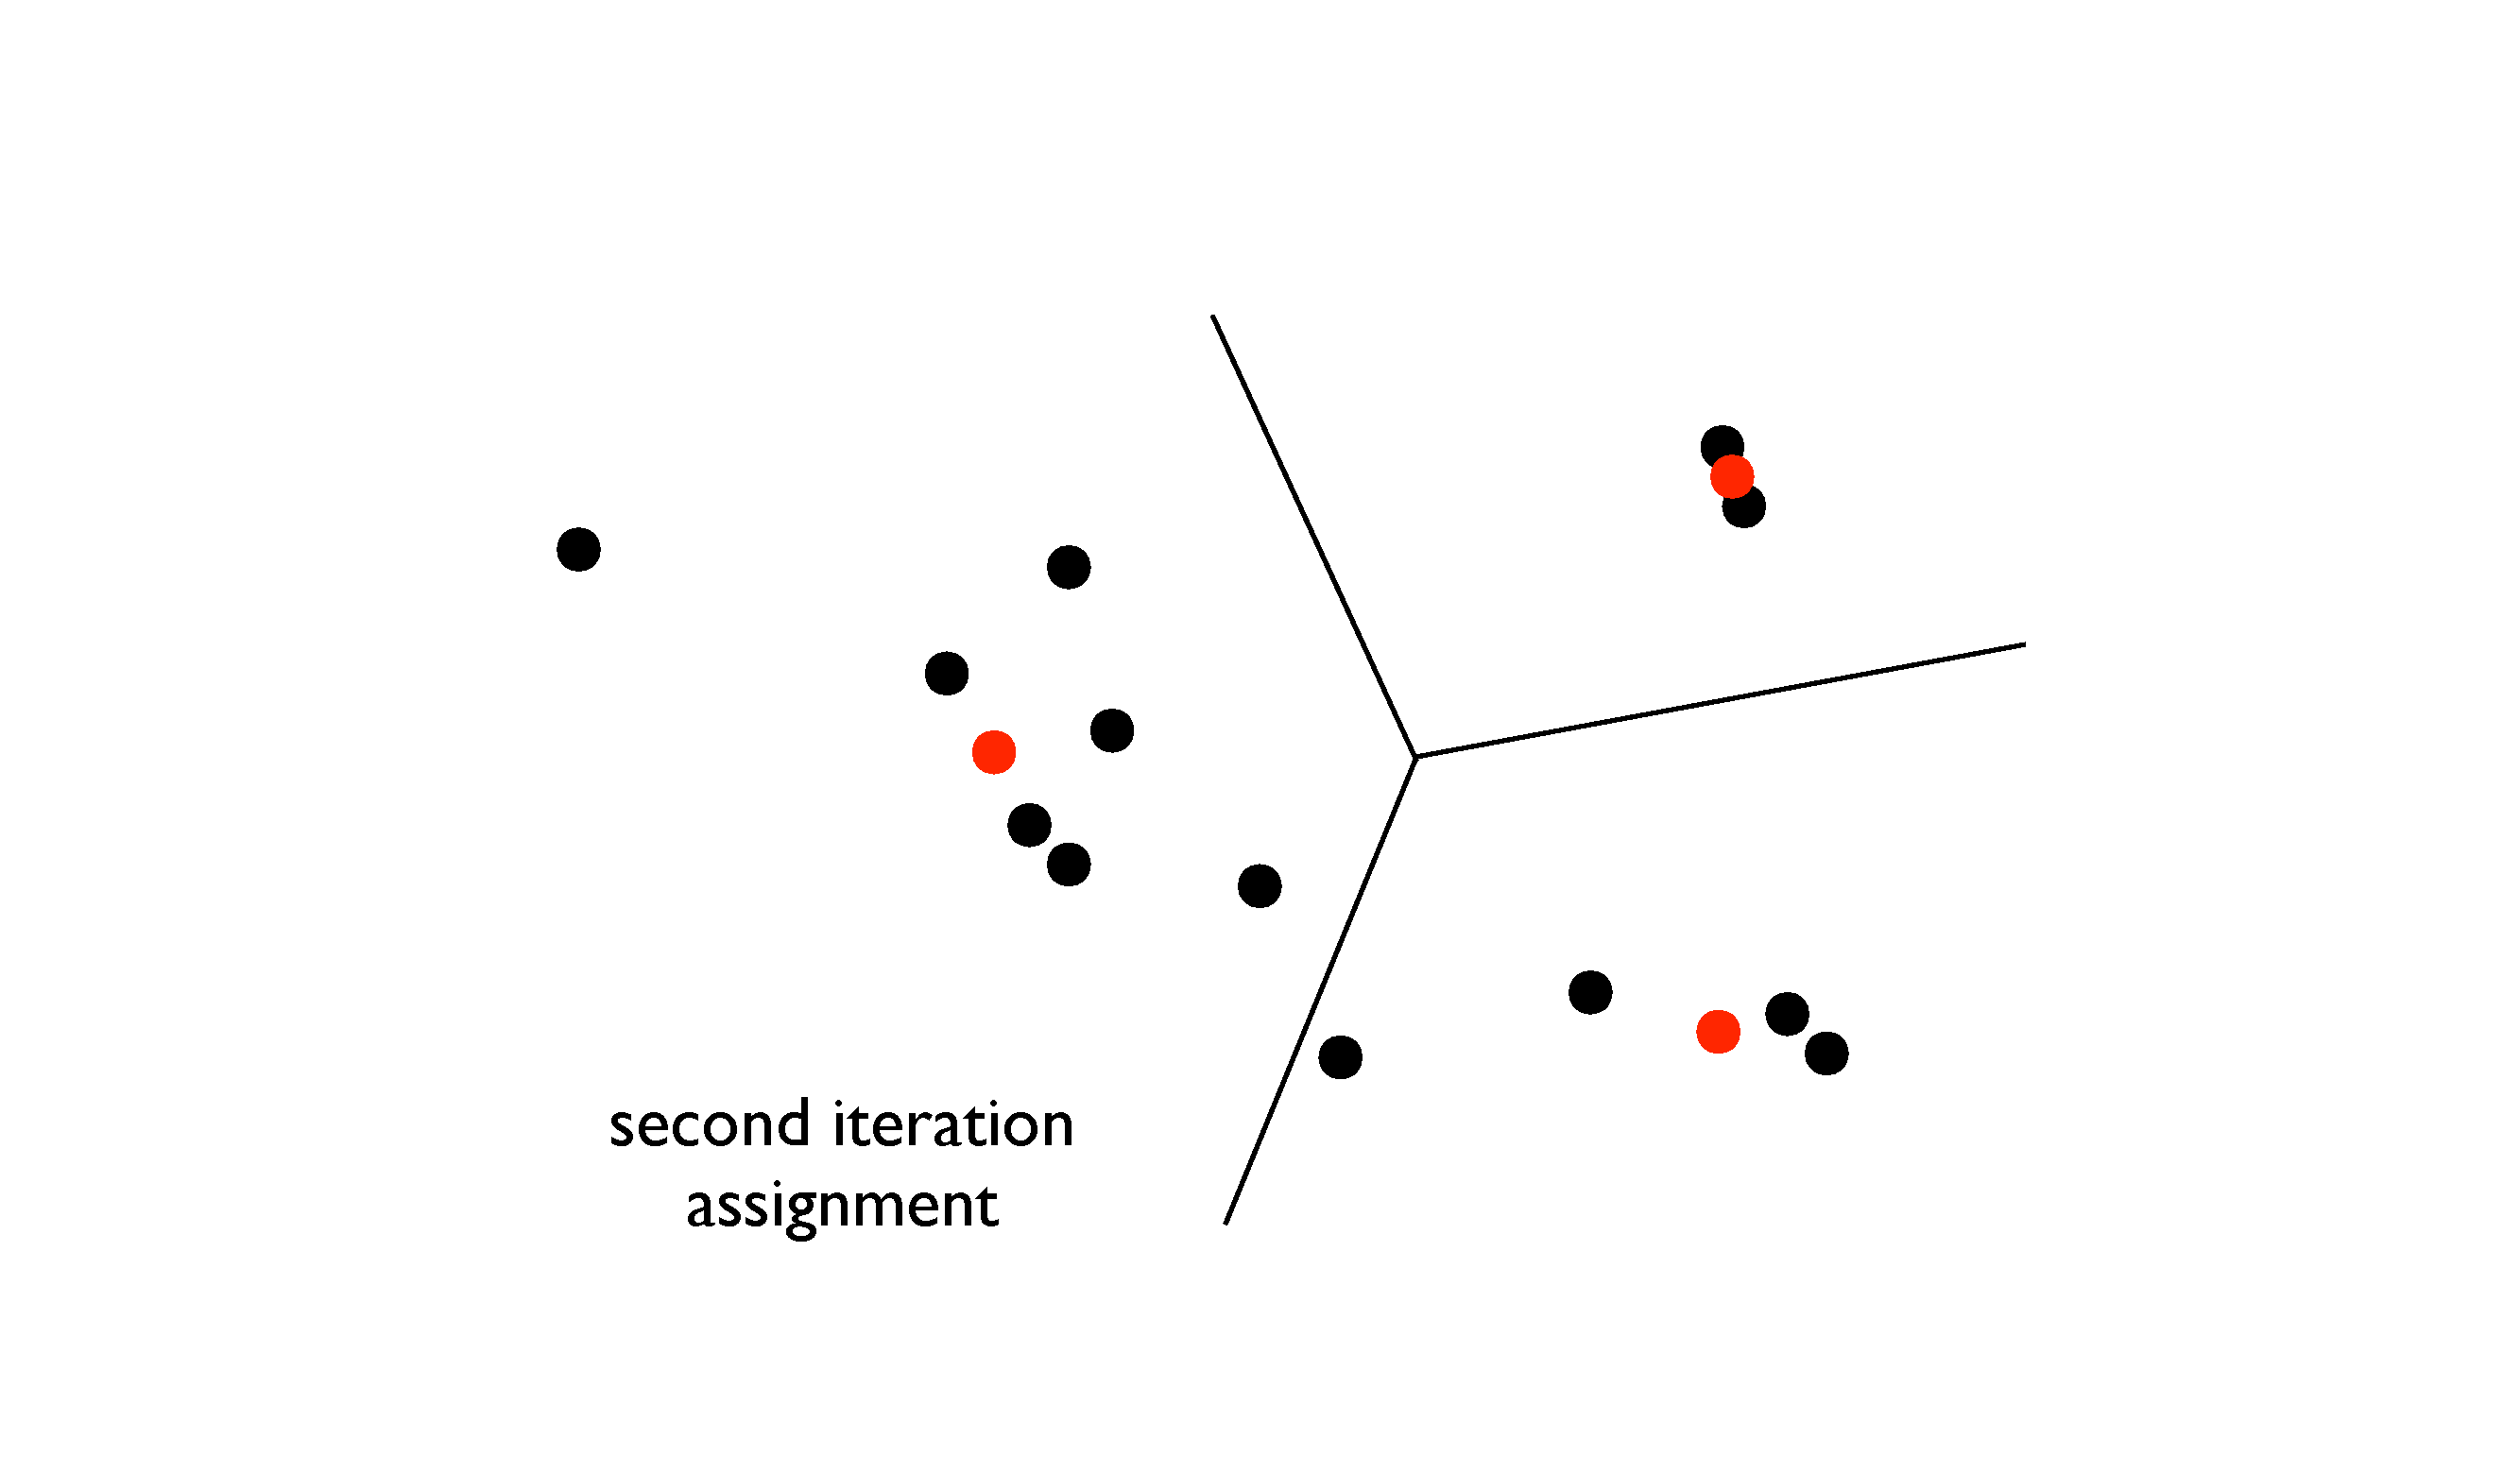
\includegraphics[scale=0.4]{kmeans-points-assign2.pdf}
\end{figure}

\begin{figure}[H]
    \caption{Second iteration centroid adjustment}
    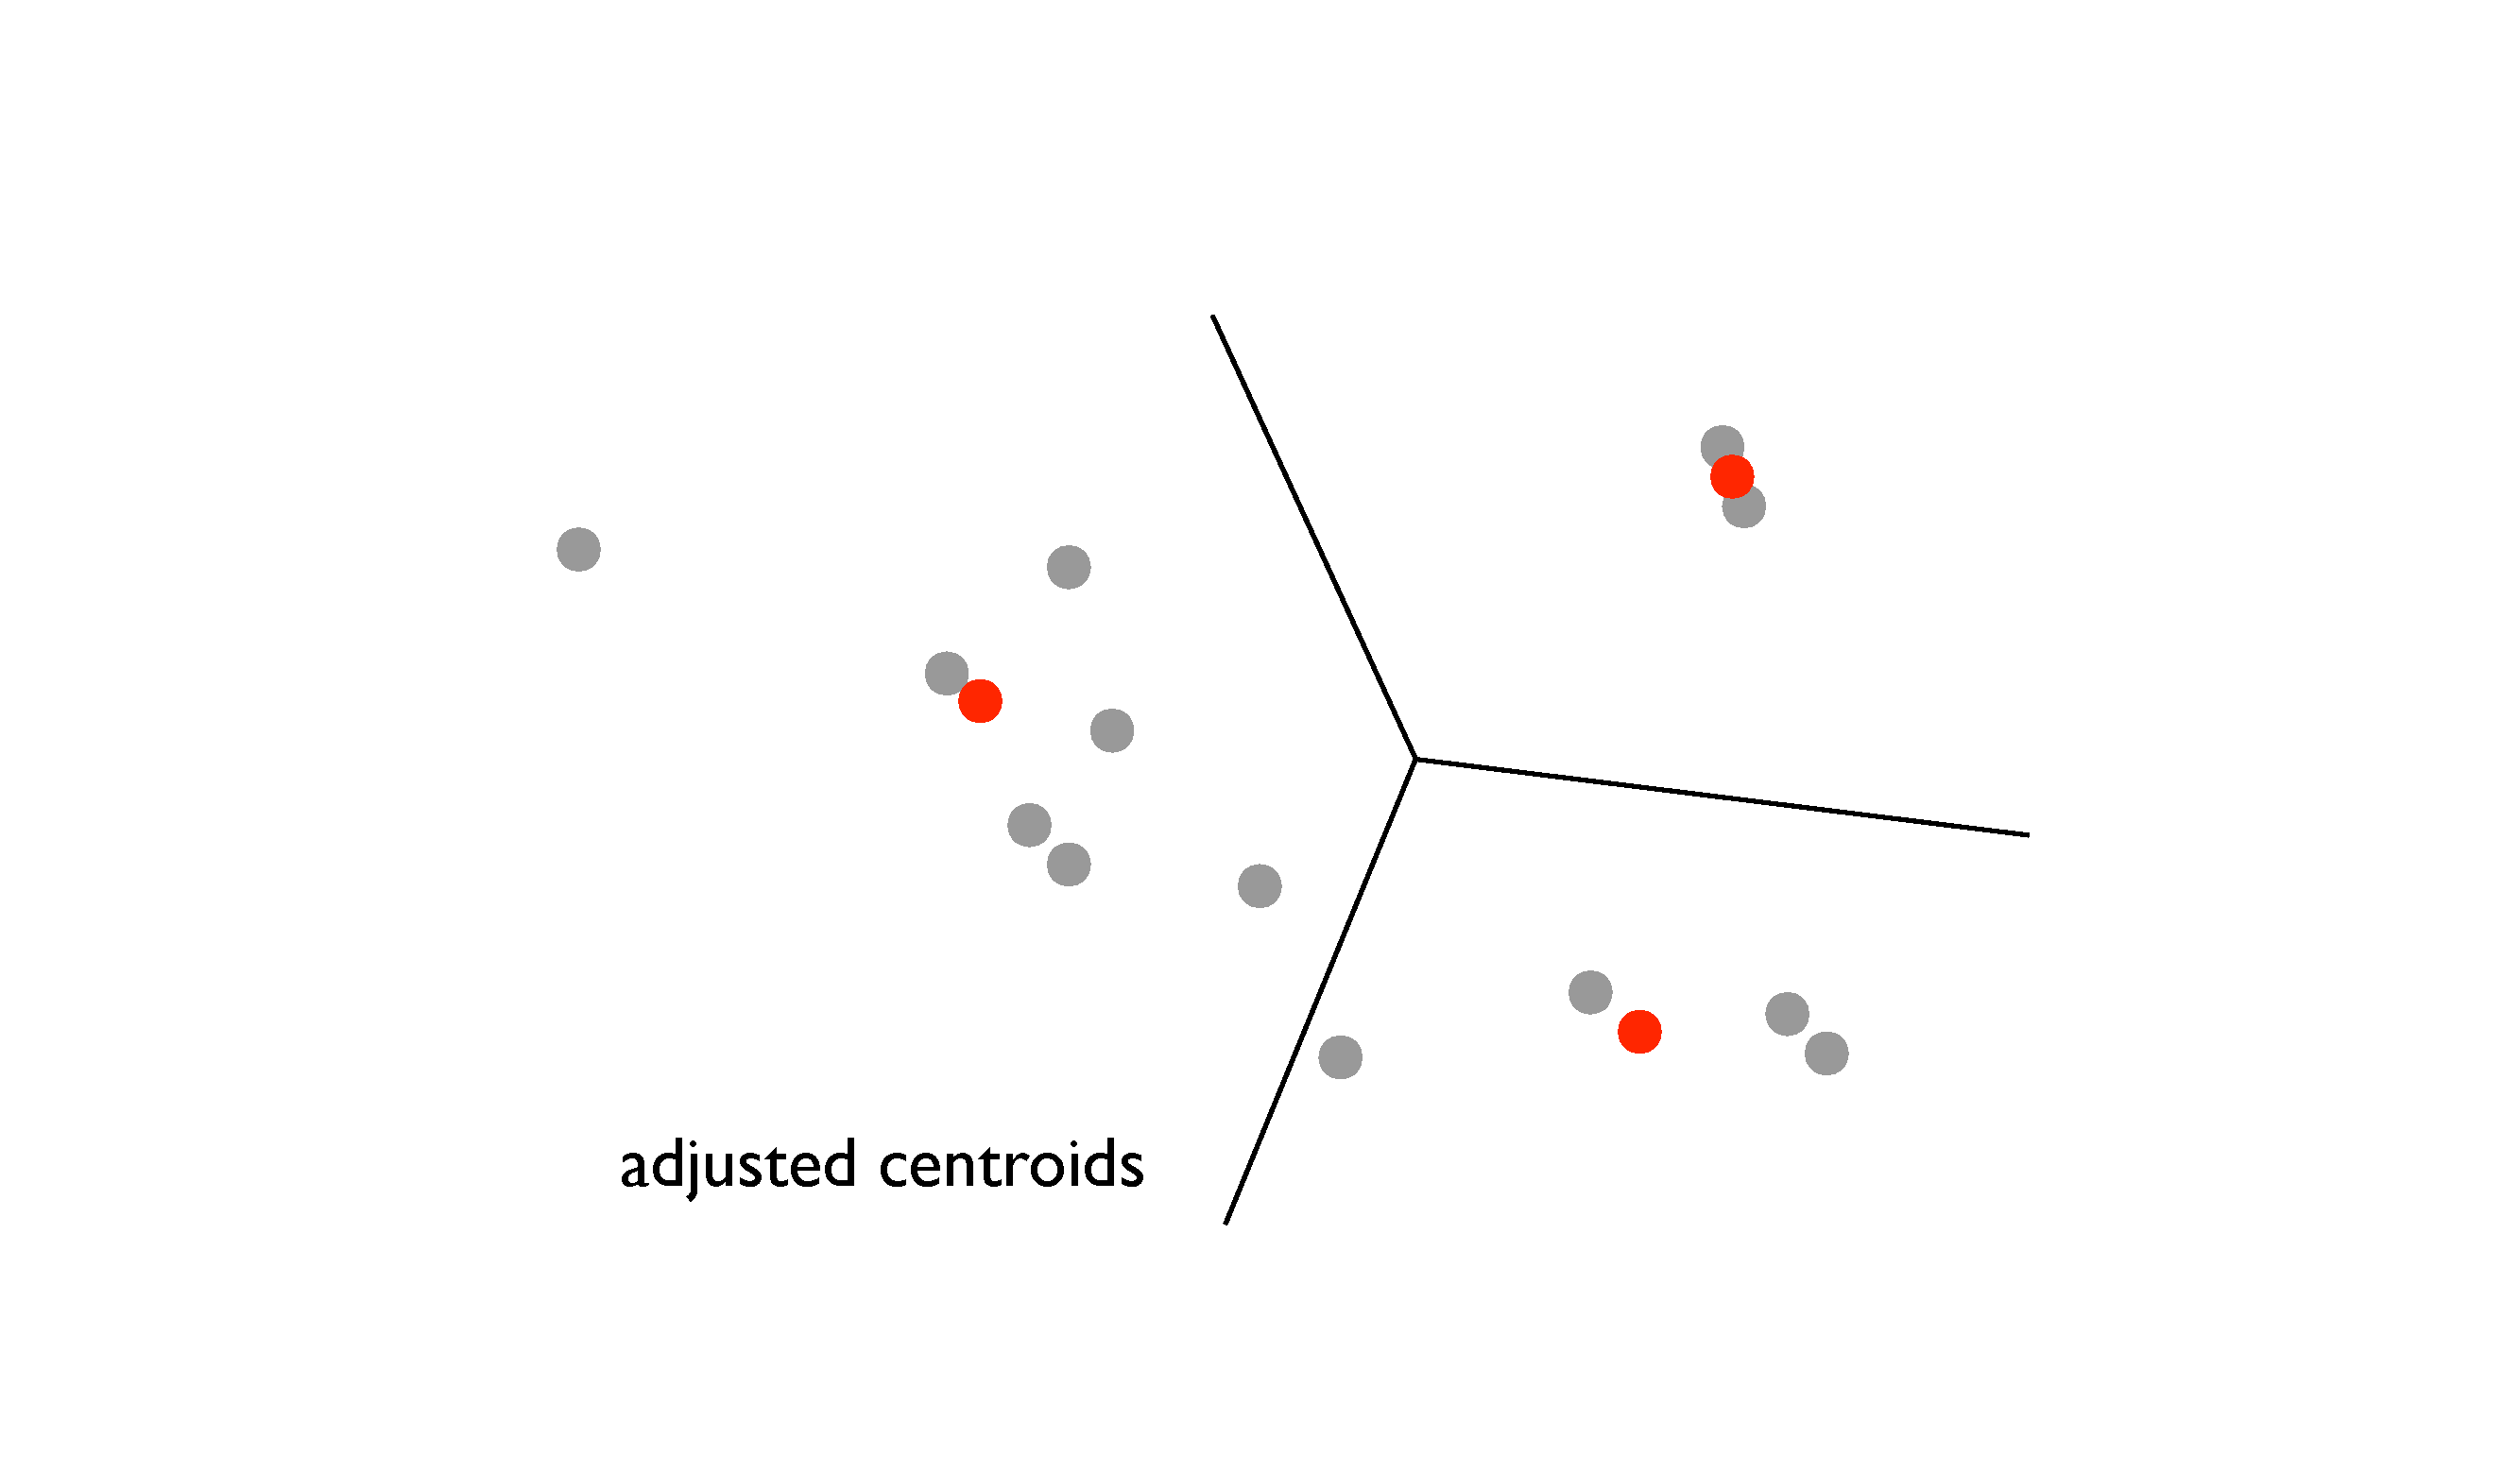
\includegraphics[scale=0.4]{kmeans-points-adjust2.pdf}
\end{figure}

\pagebreak

\subsection{Algorithm}

The pseudocode for the algorithm described above is:

\begin{algorithmic}[1]
    \State $Centroids\gets select\; k\; points \in Points$
    \While{not done}
        \For{$c \in Centroids$}
            \State $Clusters[c]\gets \emptyset$
        \EndFor
        \For{$p \in Points$}
            \State $d_{min}\gets \infty$
            \For{$c \in Centroids$}
                \State $d\gets dist(p, c)$
                \If{$d < d_{min}$}
                    \State $d_{min}\gets d$
                    \State $c_{min} \gets c$
                \EndIf
            \EndFor
            \State $Clusters[c_{min}]\gets Clusters[c_{min}] \cup \{p\}$
        \EndFor
        \State $Centroids\gets \emptyset$
        \For{$C \in Clusters$}
            \State $Centroids\gets Centroids \cup \{mean(C)\}$
        \EndFor
    \EndWhile
\end{algorithmic}

The crucial details in the algorithm are:
\begin{enumerate}
    \item centroid initialization: how are the $k$ points selected to become
        centroids at the beginning?
    \item stopping condition: how long do we need to do the point assignment
        and centroid adjustment?
\end{enumerate}
These two questions have a variety of solutions each of them resulting in a
slightly different version of the algorithm, but with mostly similary results.

\subsection{Initialization}
Selecting the first $k$ points to become centroids, or ``seeding'' as it is
also known is the single most important factor in getting a high-quality
clustering.

\subsubsection{Random selection}
The simplest solution is to simply select $k$ points of the $n$ randomly. This
produces a seed but has no real guarantees about what these points are.
For a good quality clustering, assuming there are $k$ real clusters and we wish
to identify them, the seeds should ideally come from the $k$ clusters and no
two seeds should come from the same clusters.
If this is true, because we assumed the clusters really do exist in the data,
the cluster assignment will set nearly all the points in the right cluster in
just a few steps.
The downside of this approach is illustrated in the figure below. There, two
seeds are selected from the same real cluster, causing it to be split among the
two k-means clusters (red and yellow). This means, another cluster (the blue
one) will have to contain points from two real clusters.
\begin{figure}[H]
    \caption{Here is a case where the random initialization failed and a
    single real cluster was split between the yellow and red k-means clusters}
    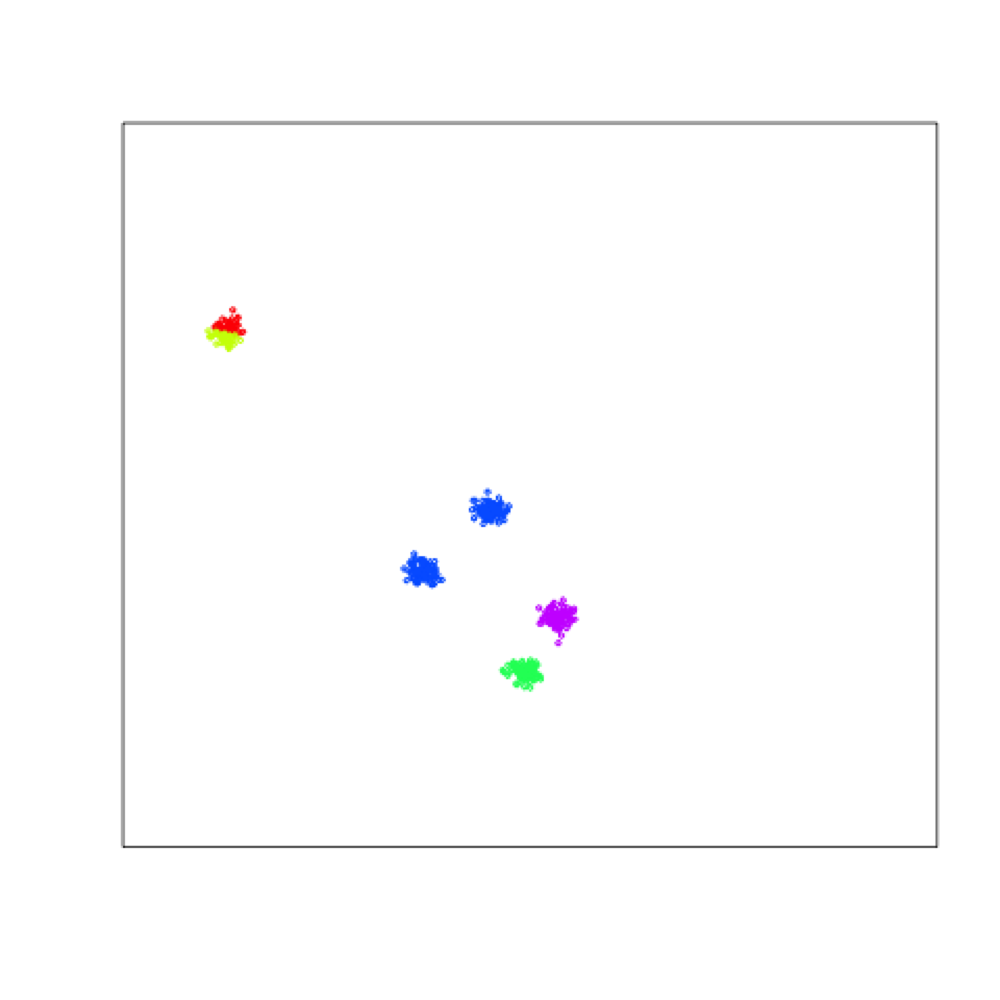
\includegraphics[scale=0.7]{kmfail.png}
\end{figure}
Additionally, like many machine learning algorithms that only result in locally
optimal solutions, k-means benefits from multiple restarts. Multiple restarts
are even more important as this makes it nearly impossible to not have a good
set of initial centroids.

\subsubsection{k-means++}
There are ways of improving the selection of centroids through the intuitive
idea that we want to have seeds that are as far apart to each other as
possible. This effectively eliminates the problem of having two seeds in the
same cluster. While there are multiple ways of doing this, the most widely used
one probably being \cite{Arthur2007}. The approach I implemented is described
in \cite{Ostrovsky} and is summarized below. In \cite{Ostrovsky}, Ostrovsky et.
all introduce a new condition, called {\it $\epsilon$-separability} that
formalizes what data should look like for a good clustering to exist and give
an new way of sampling the initial centroids with provably-good guarantees.
This sampling is fairly similar to k-means++ and they show how it can produce a
constant-factor approximation of the optimal clustering with just one Lloyd
step provided the data is $\epsilon$-separable.

From an implementor's perspective, checking if the data is indeed
$\epsilon$-separable is of little interest. We would need to know the optimum
clustering cost for $k$ clusters and $k - 1$ clusters and if we could compute
those, we'd just do it directly.
The new sampling method however, is useful and we describe it below (based
on section 4.1.1 in \cite {Ostrovsky}).

First, we select two centroids, $c_1$ and $c_2$ with probability proportional
to $dist(c_1, c_2)$. \cite{Ostrovsky} uses $dist({\bf x}, {\bf y}) = ||{\bf x -
y}||_2^2$ as the distance measure, but as explained above, we generalize this
in the implemetation to any user supplied function. We now have the first 2
centroids.

Then, to select the $(i + 1)$-th centroid, call the $i$ already selected centers,
$\mathbf{c}_1 \ldots \mathbf{c}_i$. The new point is selected randomly with
probability proportional to $\min_{j \in \left\{ 1 \ldots i \right\}}
dist(\mathbf{x}, \mathbf{c}_j)$.

\subsection{Convergence}

As with most iterative machine learning algorithms, the main k-means step is
performed multiple times. We stop the algorithm after:
\begin{itemize}
    \item a fixed number of iterations, this is usually an upper bound
    \item a quality metric plateaus (in this case, total cost), meaning that
        it stops decreasing after a few iterations
    \item no points change cluster assignment
\end{itemize}

\subsection{Number of clusters}

Clustering is a very broad and somewhat loosely defined problem in general. In
fact, \cite{why} jokingly remarks that ``clustering is in the eye of the
beholder''.
While we have formalized the problem in section 2, by explicitly stating that
we are given $n$ $d$-dimensional points and the distance measure $dist$, we
also assume to be given $k$.

This might be true, but most of the time in practice it isn't. Typically
however, this being an unsupervised learning problem, there is no ground truth.
This implies that we can't know what the value of $k$ actually is, and
sometimes we don't particularly care (notably, when using clustering to sample
our original data set).
One well known way of addressing this is the ``Elbow Method'', where one tries
clustering the points with different values of $k$ and plots the total cost
$T_c$ as a function of $k$. The total cost should go down as more clusters are
available, because ``real'' clusters in the data have too few clusters to
properly represent them, until after reaching this point, the cost plateaus
because more clusters fit the real clusters exactly.

\subsection{Outliers}

Real data is often messy: it's put together from various data sources by (buggy)
algorithms and (falible) humans and errors are likely. These errors look like
outliers in the data where one of the dimensions is much different than the
rest. In an unlucky case, these outliers migh even be fairly close together,
warranting the question of whether they should be thought of as a cluster
themeslves.

In the figure below, suppose we're convinced that the 3 points at the bottom
right are outliers and that there are only 2 clusters in the data.
Then, the reasonable thing to do, is discard them and not have them be part of
any cluster.

\begin{figure}[H]
    \caption{Data set where outliers have skewed the centroids}
    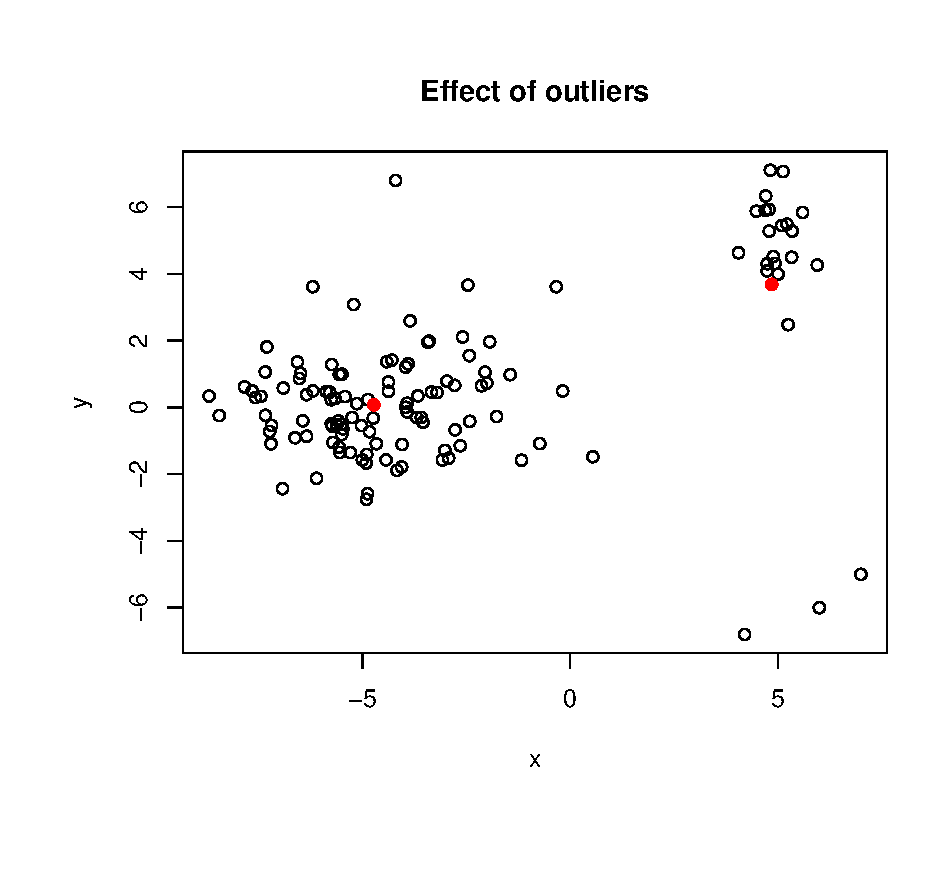
\includegraphics[scale=0.7]{outliers.pdf}
\end{figure}

That's not possible with standard k-means as every point is part of exactly one
cluster and contributes to that cluster's mean. This is why in the figure, the
centroid of the cluster in the top-right is skewed downwards towards the three
outliers at the bottom-right. The only thing to do here is to manually remove
the outliers which is plausible for a small data set, but impossible for even a
medium-sized one.

The solution, lifted from \cite{Ostrovsky} modifies the centroid update
operation. Instead of taking all the points assigned to a cluster into account
when computing the new centroid, onle points that are within a ball (in the
topological sense) are averaged.
The radius of this ball is fraction (user-configurable in practice) of the
smallest inter-cluster distance within the clustering. This ensures that only
points close to the cluster's ``core'' play a role in the adjustment of its
centroid.

\subsection{Algorithm Complexity}

A major consideration not treated up until now in this paper is the complexity of
the algorithm. While the number of iterations is highly-dependent on the
initial centroid seeding and the particular shape of the data, for a given
k-means step, the two main operations take:
\begin{enumerate}
    \item point to cluster assignment: for each of the $n$ points, go through
        all $k$ centroids and compute the distance between the $d$-dimensional
        vectors. This step is therefore $O(n k d)$.
    \item centroid adjustment: the points are partitioned across $k$ clusters,
        but they are essentially summed up and divided by their count in each
        cluster. Therefore, this step is $O(n d)$.
\end{enumerate}

So, for a given step, the total cost is $O(n k d + nd) = O(n k d)$. Each of
these variables could conceivable be reduced.

\begin{enumerate}
    \item $n$: The data could be downsampled, thereby reducing
        $n$.  Downsampling needs to take into account the particular distribution 
        of the data and preserve it well-enough for
        the final clustering. This is the route taken indirectly by the
        streaming k-means approach described in section 9.
    \item $d$: The vectors' dimensionality could be reduced through standard
        techniques like Principal Component Analysis.
    \item $k$: Searching for the nearest neighbor among all the centroids is
        usually not a significant expense when $k$ is small. For most
        ``classical'' clustering applications, $k$ is less than 100. However,
        especially when using clustering as a way of approximating data, or
        when dealing with web-scale data, $k$ can be much larger, potentially
        on the order of millions. And even if it isn't, being a multiplicative
        constant is reason enough to want to reduce it.
        This can be achieved through approximate nearest-neighbor searches.
\end{enumerate}

\subsubsection{Approximate nearest-neighbor search}

There are many approaches to this problem, some of which are surveyed by Riegger
in \cite{Riegger2010}.
The one we chose is based on the Johnson-Lindenstrauss Lemma by W. Johnson and
J. Lindenstrauss in \cite{jl}, for which an
elementary proof is given by Dasgupta et. all in \cite{Dasgupta2003}. Citing
directly from their abstract,

\begin{quote}
    A result of Johnson and Lindenstrauss shows that a set of $n$ points in
    high dimensional Euclidean space can be mapped into an $O(\log
    \frac{n}{\epsilon})$-dimensional Euclidean space such that the distance
    between any two points changes by only a factor of $(1 \pm \epsilon)$.
\end{quote}

The mapping can be obtained by simply sampling $d_r = O(\log \frac{n}{\epsilon})$
$d$-dimensional random vectors from $\mathcal{N}(0, 1)$ and then
normalizing each vector \cite{Dasgupta2003}.

Arranging these $d_r$ vectors into a $d_r \times d$ sized
projection matrix, $P$, multiplying $A$ by a $d$-dimensional vector
$\mathbf{v}$ results in a $d_r$-dimensional vector, $P \mathbf{v}$.
This is random-projection based dimensionality reduction.

The main problem with nearest-neighbor searches is their inability to
narrow-down the candidate set. On scalar data, the two main approaches for
fast searching are based either on a total ordering of the elements and
binary-search like approaches or a hashing function and use a hash-table.

Vectors in $\mathbf{R}^d$ are not intuitively comparable, and defining an
order of the dimensions doesn't work well. To see why, consider points
$\mathbf{a, b, c} \in \mathbf{R}^d$ and the L1 norm of the difference of two
vectors as the distance measure. If the order of the dimensions is from 1
to $d$, the ordering of the vectors is equivalent to lexicographic. Suppose
$\mathbf{b} = [b_1, \ldots, b_d]^T = [a_1 + \epsilon, \ldots, a_{d - 1} + \epsilon, a_d + \delta_b]^T$ and $\mathbf{c} = [c_1, \ldots, c_d]^T = [a_1 + 2 \epsilon, a_2, a_3 + \epsilon \ldots a_{d - 1} + \epsilon, a_d + \delta_c]$.
Under the chosen distance measure, $||\mathbf{a} - \mathbf{b}||_1 = (d - 1)
\epsilon + \delta_b$ and $||\mathbf{a} - \mathbf{c}||_1 = (d - 1) \epsilon +
\delta_c$.
In this case the first $d-1$ dimensions are not relevant to the comparison,
yet, in under the ordering $\mathbf{b}$ would come before $\mathbf{c}$ and
worse, according to the chosen distance measure $\mathbf{c}$ could even be closer to
$\mathbf{a}$ (depending on $\delta_b$ compared to $\delta_c$).
This shows that this type of ordering, doesn't guarantee the ordering of
distances, making it useless for nearest-neighbor searches.

Hashing a vector would result in a scalar that's close to uniformly distributed
in some interval so that the resulting hash table is as close to balanced as
possible. The issue here is that hashing two similar vectors with a typical
good hashing function results in them being far away from each other.
This makes trying out more than 1 candidate infeasible and therefore k-nearest
neighbor searches impossible.

Random projections offer a better approach. Consider figure 9, below.
Call the line such a projection vector, $\mathbf{p}$. The line is the direction
of the projection vector, not the vector per se (the vector is normalized to
unit length). Each dot then, represents another vector in 2D space.
Projecting a vector $\mathbf{a}$ on to another vector $\mathbf{p}$, visualized 
here as projecting a point on to a line, results in a vector in the same
direction as $\mathbf{p}$ and with magnitude $|\mathbf{a}| |\mathbf{p}| \cos \angle(\mathbf{a}, \mathbf{p})$.
Since all the resulting vectors are in the same direction, just the magnitudes (that
are scalar!) need to be compared.

Note that vectors that are close in the original space, will result in comparable
magnitudes. This is the very fact that enables the Johnson-Lindenstrauss lemma.
However, vectors that are far away in the original space, could also map to similar
magnitudes (like the top most 2 projections in figure 9). This means that
closeness in the original space guranatees close scalars, but the converse is
not true.
There could even be points that are farther away from a point in the original space
that project more closely to a it than points that are closer to the said point.

This uncertainty gives rise to the approximate nature of the search. The
closest neighbor is likely close by, but if the direction of the projection is
particularly unlucky, it can be completely ignored in favor of points that are
farther away.

\begin{figure}[H]
    \caption{An example of the resulting projections on to a random vector}
    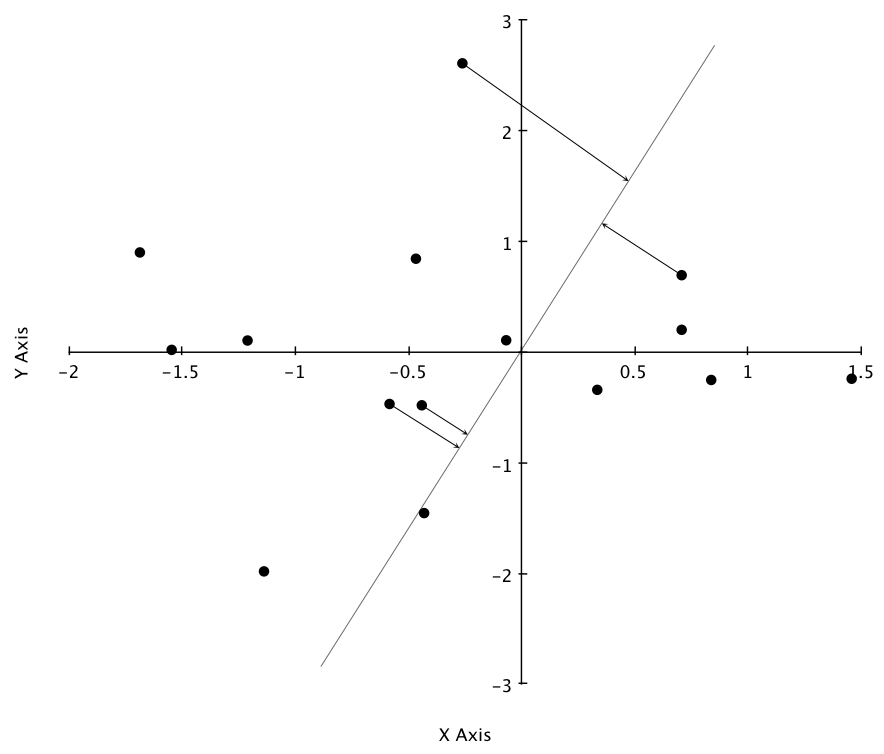
\includegraphics[scale=0.8]{proj.png}
\end{figure}

In fact the approximation becomes better as more directions are considered and the
Johnson-Lindenstrauss lemma gives explicit bounds for the number of projections
required for required given quality of the answer.

In figure 10, even when using 1 projection, for low-dimensional spaces, the
probability of finding the best neighbor directly is quite substantial.

\begin{figure}[H]
    \caption{}
    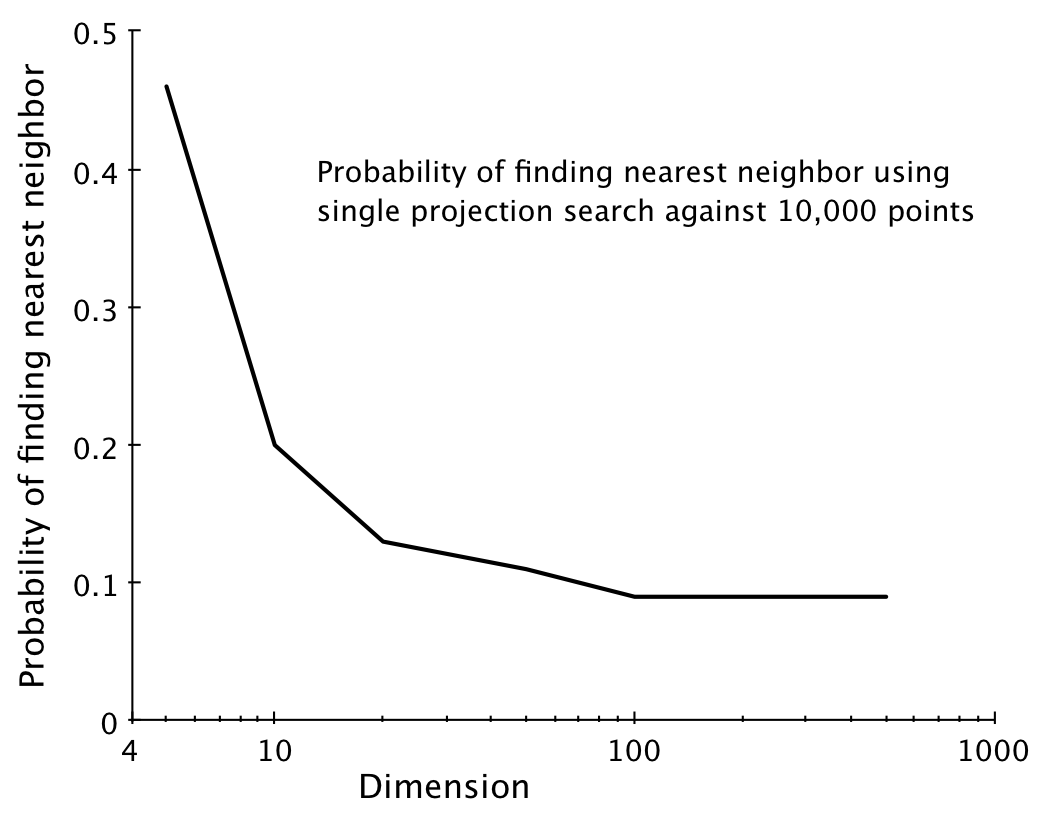
\includegraphics[scale=0.7]{qualproj.png}
\end{figure}

For the closest $k$ neighbors the strategy now becomes selecting a ball of size $b$ around where
the projected query is for each of the $p$ projections, merging all of these
balls into a candidate set of size $2bp$ and searching in this new set.

This new set only has $2bp$ points in it which should be a lot less than the
original number of vectors to search through. The distance here are computed
completely.
The size of the ball, $b$ and the number of projections $p$ are the parameters.

\begin{algorithmic}[1]
    \State $Candidates \gets \emptyset$
    \For{$\mathbf{p} \in$ $Projection$s}
        \State $\mathbf{pq}\gets$ project query on to $\mathbf{p}$
        \State $\mathbf{c}\gets$ closest neighbor of $\mathbf{pq}$ induced by $\mathbf{p}$
        \State $Candidates\gets Candidates$ $\cup$ ball of size $b$ around $\mathbf{c}$
    \EndFor
    \State keep closest $k$ from $Candidates$ by computing the actual distances
\end{algorithmic}

\section{Large scale}

\section{Batch processing: MapReduce}

\section{Online processing: Storm}

\section{k-means as a MapReduce}

\subsection{Algorithm}

\subsection{Discussion}

\subsubsection{Multiple passes through the data}

\subsubsection{Random initialization}

\section{Making big data small}

\section{Streaming k-means}

\subsection{Algorithm}

\subsection{Discussion}

\section{Clustering big data: MapReduce}

\subsection{Mahout implementation}

\section{Clustering big data: Storm}

\subsection{Storm prototype}

\section{Results}

\subsection{Quality}

\subsubsection{Data sets}

\subsubsection{Quality measures}

\subsubsection{Experiment}

\subsubsection{Discussion}

\subsection{Speed}

\subsubsection{Data sets}

\subsubsection{Cluster}

\subsubsection{Experiment}

\subsubsection{Discussion}

\section{Conclusion}


\begin{thebibliography}{99}
    \bibitem{Arthur2007} Arthur, D., \& Vassilvitskii, S. (2007). k-means++ : The Advantages of
        Careful Seeding. Proceedings of the eighteenth annual ACM- …, 8, 1–11.
        Retrieved from http://dl.acm.org/citation.cfm?id=1283383.1283494

    \bibitem{Ostrovsky} Ostrovsky, R. (n.d.). The Effectiveness of Lloyd-type
        Methods for the k-Means Problem, 1–18.

    \bibitem{why} Why so many clustering algorithms? - A position paper SIGKDD
        explorations, Vol. 4, No. 1. (June 2002), pp. 65-75 by Vladimir
        Estivill-Castro

    \bibitem{Indyk} Indyk, P., \& Motwani, R. (n.d.). Approximate Nearest Neighbors :
        Towards Removing the Curse of Dimensionality, 604–613.

    \bibitem{Riegger2010} Riegger, P. M. (2010). Literature Survey on Nearest Neighbor Search and Search in Graphs, (2300), 1–36.

    \bibitem{jl} W. B. Johnson and J. Lindenstrauss, Extensions of Lipschitz maps into a Hilbert space, Contemp Math 26 (1984), 189–206.

    \bibitem{Dasgupta2003} Dasgupta, S., \& Gupta, A. (2003). An elementary proof of a theorem of Johnson and Lindenstrauss. Random Structures and Algorithms, 22(1), 60–65. doi:10.1002/rsa.10073
\end{thebibliography}
\end{document}
